\section{Efficient Maintenance With Sampling} \label{sampling}
%\reminder{Make sure that we do a good survey on ``sampling from a view" and discuss them in the related work, e.g., [Frank et al., VLDB 86], [Nirkhiwale et al., VLDB 13]}
In the previous section, we formalized the procedure of taking a uniform sample of rows $\hat{S}$, and ``cleaning" it to produce a corresponding uniform sample of the up-to-date view $\hat{S'}$.
This procedure is not unique and there are both efficient and inefficient (i.e., not any easier than updating the entire materialized view) ways to accomplish this. 
For example, a naive solution to derive a sample $\hat{S'}$ is to just apply the maintenance strategy and then sample.
However, this does not make the maintenance of the sample any more efficient.

Ideally, we want to integrate the sampling into the maintenance strategy $\mathcal{M}$ so that expensive operators
need not operate on the full data.
In this section, we discuss how to efficiently derive $\hat{S'}$ and the conditions under which
maintaining $\hat{S'}$ is much cheaper than maintaining the entire view $S'$.

\subsection{Uniform Sampling on Views}
We first discuss some of the difficulties with uniform sampling.
%In this work, we focus on result estimation on uniform samples of views. \reminder{You have already explained uniform sampling in Sec 3.2.}
For a sampling ratio $m$, we call a sample view $\hat{S'}$ a uniform sample of $S'$, under the following condition:

\begin{definition}[Uniform Sample] We say the relation $\hat{S'}$ is a \emph{uniform sample} of $S'$ if
\begin{enumerate}[label=(\arabic*),itemsep=1pt]
\item $\forall s \in \hat{S'} : s \in S'$;
\item $Pr(s_1 \in \hat{S'}) =  Pr(s_2 \in \hat{S'}) = m$.
\end{enumerate}
\end{definition}

A traditional ``coin-flip" sampling algorithm is not suited for this property as it is known that such sampling commutes very poorly with many relational operations such as joins and aggregates \cite{chaudhuri1999random}.
Recall, the view in our example \textsf{countView}. 
Suppose, we sampled from the base relation \tbl{Log}, and then applied the view definition to the sample to form the ``delta view".
The ``delta view" would have a mix of missing videos (\textsf{videoId} is not in the sample) and rows with incomplete aggregates (not all of the videos with \textsf{videoId} are in the sample).
However, this is not what we require since it is not a uniform sample of the rows in the view. 

To get a uniform sample of a view, the main problem is that for every row sampled in the view, our sampling technique needs to include all of the rows in sub-expressions that contribute to its materialization.
Achieving this requires a definition of lineage; traceable, unique identification for rows.

\subsection{Identification With Row Lineage}
\label{lin}
Lineage has been an important tool in the analysis of materialized views \cite{DBLP:journals/vldb/CuiW03} and in approximate query processing \cite{DBLP:conf/sigmod/ZengGMZ14}. %\reminder{Add Kai into acknownledgement for helping us with problem formulation. }
We recursively define a set of consistent primary keys for all nodes in the expression tree:
\begin{definition} [Primary Key]
For every relational expression $R$, we define the primary key of every expression to be:
\begin{itemize}[noitemsep]
\item Base Case: All relations (leaves) must have an attribute $p$ which is designated as a primary key. That uniquely identifies rows.
\item $\sigma_{\phi}(R)$: Primary key of the result is the primary key of R 
\item $\Pi_{(a_1,...,a_k)}(R)$: Primary key of the result is the primary key of R. The primary key must always be included in the projection.
\item $\bowtie_{\phi (r1,r2)}(R_1,R_2)$: The primary key of the result is the union of the primary keys of $R_1$ and $R_2$. 
\item $\gamma_{f,A}(R)$: The primary key of the result is the group by key $A$ (which may be a set of attributes).
\item $R_1 \cup R_2$: Primary key of the result is the primary key of~R
\item $R_1 \cap R_2$: Primary key of the result is the primary key of~R
\item $R_1 - R_2$: Primary key of the result is the primary key of~R
\end{itemize}
\end{definition}
This definition of a primary key for a relational expression, allows us to trace the primary key through the expression tree.
%Our definition of the primary key is also constructive; that is, if an expression has a null primary key then we modify every projection operation to ensure that primary key of the subrelation is never projected out.

\subsection{Hashing Operator}
\label{push}
If we have a deterministic way of mapping a primary key defined in the previous subsection to a sample, we can also ensure that all contributing expressions are also sampled. 
To achieve this we use a hashing procedure.
Let us denote the hashing operator $\eta_{a, m}(R)$. 
For all tuples in R, this operator applies a hash function whose range is $[0,1]$ to primary key $a$ (which may be a set) and selects those records with hash value less than or equal to $m$.
If the hash function is sufficiently uniform, then $h(a) \le m$ samples close to a fraction $m$ of the tuples.
%This definition is without loss of generality for uniform hash function, as if we have a hash function whose range is the set of integers (as implemented in MySQL or Apache Hive) we can take the absolute value and divide by the maximum integer mapping this range back $[0,1]$. 

To achieve the performance benefits of sampling, we push down the hashing operator through the query tree.
The further that we can push $\eta$ down the expression tree, the more operators can benefit from the sampling.
However, it is important to note that for some of the expressions, notably joins, the push down rules are more complex. 
It turns out in general we cannot push down even a deterministic sample through those expressions.
We formalize the push down rules below:
\begin{definition}[Hash Pushdown]
Let $a$ be a primary key of a materialized view. The following rules can be applied to push $\eta_{a, m}(R)$ down the expression tree of the maintenance strategy. 
\begin{itemize}[noitemsep]
\item $\sigma_{\phi}(R)$: Push $\eta$ through the expression.  
\item $\Pi_{p,[a_2,...,a_k]}(R)$: Push $\eta $ through if $a$ is in the projection.
\item $\bowtie_{\phi (r1,r2)}(R_1,R_2)$: Blocks $\eta $ in general. There are special cases below where push down is possible.
\item $\gamma_{f,A}(R)$: Push $\eta $ through if $a$ is in the group by clause $A$.
\item $R_1 \cup R_2$: Push $\eta $ through to both $R_1$ and $R_2$
\item $R_1 \cap R_2$: Push $\eta $ through to both $R_1$ and $R_2$
\item $R_1 - R_2$: Push $\eta $ through to both $R_1$ and $R_2$
\end{itemize}
\end{definition}
In special cases, we can push the hashing operator down through joins. 
Given the hash function $\eta_{a, m}(R)$:

\textbf{Equality Join Key: } If the join is an equality join and $a$ is one of the attributes in the equality join condition $R_1.a = R_2.b$, then $\eta$ can be pushed down to both $R_1$ and $R_2$. On $R_1$ the pushed down operator is $\eta_{a, m}(R_1)$ and on $R_2$ the operator is $\eta_{b, m}(R_2)$.

\textbf{Primary Key Many-to-one: } If we are hashing the primary key of the result of a Foreign-Key join, the push down is possible. We have a join with two relations $R_1$ and $R_2$ and we know that for every $r_1 \in R_1$ there is exactly one $r_2$ in $R_2$ that satisfies the join condition. Based on the lineage rules defined earlier, the primary key is the union of the sets of primary keys of $R_1$ and $R_2$. However, since we know that there is only 1 $r_2$ for every $r_1$, it is equivalent to hash just the primary key of $R_1$. Thus, $a$ in our hash function is the primary key of a Foreign-Key join, then we can push it down to $R_1$, $\eta_{a, m}(R_1)$. 

\textbf{(Semi/Anti)-Join: } Similarly, if we are hashing the primary key of a semi-join, we can always push $\eta$ down $R_1$. For anti-joins we can push $\eta$ down because we can rewrite the node as $R_1 - (R_1 \ltimes R_2) $ and apply the pushdown rules for set difference and Semi-Joins.

\subsection{Corresponding Samples}
We showed that we can optimize a hashed maintenance plan $\eta(\mathcal{M})$ by using push-down rules.
This gives us an expression to maintain a sample of rows in the up-to-date view $S'$.
When the insertion and deletion relations $\{\Delta R_i\} \cup \{\nabla R_i\}$ are not empty, we can use
this expression to propagate changes to our sample.

One benefit of deterministic hashing is that we get the Correspondence Property (Definition \ref{correspondence}) for free.
\begin{proposition}[Hashing Correspondence]
Suppose we have $S$ which is the stale view and $S'$ which is the up-to-date view.
Both these views have the same schema and a primary key $a$.
Let $\eta_{a, m}$ be our hash function that applies the hashing to the primary key $a$.
\[
\hat{S} = \eta_{a, m}(S)
\]
\[
\hat{S'} = \eta_{a, m}(S')
\]
Then, two samples $\hat{S'}$ and $\hat{S}$ correspond.
\end{proposition}
\begin{proof}[Sketch]
Since the primary keys are key consistent between $\hat{S'}$ and $\hat{S}$, included and excluded rows are preserved by the hashing.
See the extended version for a full proof \reminder{TR}.
\iffalse
There are four conditions for correspondence:
\begin{itemize}[noitemsep]
\item 1. For every row $r$ in $\hat{S}$ that required a delete, $r \not\in \hat{S'}$
\item 2. For every row $r$ in $\hat{S}$ that required an update, $r\in \hat{S'}$
\item 3. For every row $r$ in $\hat{S}$  that was unchanged, $r \in \hat{S'}$
\item 4. For every row $r$ in $S$ but not in $\hat{S}$, $r \not\in \hat{S'}$
\end{itemize}
Condition 1 is satisfied since if $r$ is deleted, then $r \not \in S'$ which implies that $r \not\in \hat{S'}$.
Condition 2 and 3 are satisfied since if $r$ is in $\hat{S}$ then it was sampled, and then since the primary key is consistent between $S$ and $S'$ it will also be sampled in $\hat{S'}$.
Condition 4 is just the converse of 2 and 3 so it is satisfied.
\fi
\end{proof}
We will use this property in the Section \ref{correction} to get estimates for queries on the materialized view.

\subsection{Example}
We will illustrate our proposed approach on our example view \textsf{countView} (Figure \ref{exexpr}).
The maintenance strategy of this view is described in the previous section.

Based on the rules described in Section \ref{lin}, the primary key of the view is \textsf{videoId}.
The primary key for base relations \tbl{Log} and \tbl{Video} are \textsf{sessionId} and \textsf{videoId} respectively.
If we move up the tree in Figure \ref{exexpr}, the first expression in the maintenance strategy is a join making the primary key of that expression (\textsf{sessionId}, \textsf{videoId}).
Then, next there is an aggregation which groups by \textsf{videoId} making that the primary key.
This result is an equality the stale view (which has \textsf{videoId} as the primary key) making \textsf{videoId} the primary key of the epression

We can apply our sampling operator to this key, and use the pushdown rules described in Section \ref{push} to efficiently sample the maintenance strategy.
In Figure \ref{exexpr2}, we illustrate the pushdown process.
The the first operator we see in the expression tree is a projection that increments the \textsf{visitCount} in the view, and this allows
for push down since \textsf{videoId} is in the projection.
The second expression is a hash of the equality join key which merges the aggregate from the ``delta view" to the old view allowing us to push down on both branches of the tree.
On the left side, we reach the the stale view so we stop.
Since the stale view does not change, we can calculate the sample of the stale view once (eg. during periodic maintenance). 
On the right side, we reach the aggregate query (count) and since \textsf{videoId} is in group by clause, we can push down the sampling.
Then, we reach another point where we hash the equality join key allowing us to push down the sampling to the relation \tbl{LogIns} and \tbl{Video}.

\begin{figure}[t] \vspace{-2em}
\centering
 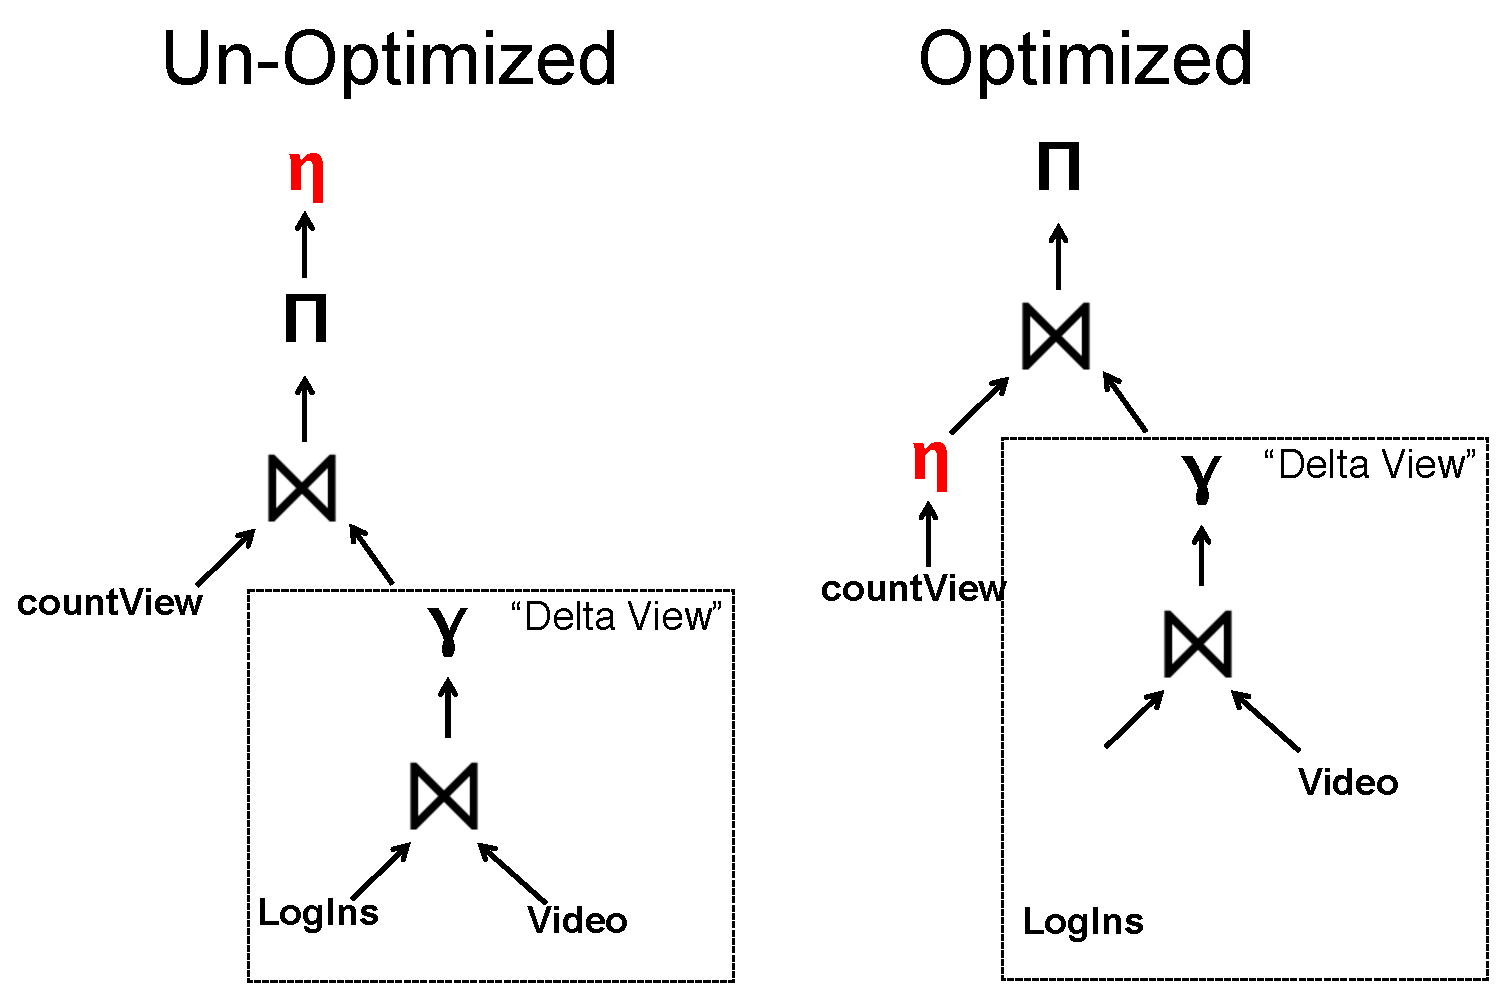
\includegraphics[scale=0.23]{figs/example_expression_tree_2.pdf} \vspace{-.25em}
 \caption{Applying the rules described in Section \ref{push}, we illustrate how to optimize the sampling of our example maintenance strategy.  \label{exexpr2}}\vspace{-1.75em}
\end{figure}

In terms of increased efficiency, since both the aggregation and joins are ``above" the sampling operator, they require less computation and less memory.


